\documentclass[10pt, a4paper]{article}
\usepackage[utf8]{inputenc}

\usepackage[left=2.5cm,right=2.5cm,top=3 cm,bottom=2cm]{geometry}

% Spanish support
\usepackage[spanish]{babel}

% Fancy authoring
\usepackage{authblk}

% Bibliography
\usepackage[backend=biber, style=numeric]{biblatex}
\addbibresource{bibliography.bib}

% Graphics
\usepackage{graphicx}
\graphicspath{{./imgs/}}

% Equations
\usepackage{amsmath} 

% Tables
\usepackage{multirow}

\title{Reconocimiento de frutas mediante visión artificial usando \textit{k-means} y \textit{k-nn}}

\author[1]{Gino Hernán Avanzini}
\affil[1]{Facultad de Ingeniería - Universidad Nacional de Cuyo}
\date{Febrero 2020, Mendoza - Argentina}


\begin{document}

\maketitle

\begin{abstract}

Se desarrolló un sistema de reconocimiento de frutas mediante el uso de técnicas de procesamiento de imagen e inteligencia artificial. Para ello se utilizó la última versión del \textit{dataset} ``Fruit 360'' junto con fotografías propias. Se realizó un trabajo de preprocesamiento de las imágenes para eliminar ruido y acentuar características para la posterior extracción de las mismas. Dichas características fueron usadas para el reconocimiento de las frutas con el uso de los algoritmos \textit{
k-means} y \textit{k-nn}. Se evalúan y comparan los resultados y se propone la adopción de uno de los dos algoritmos. 

\end{abstract}

\section{Introducción}

Bajo la directiva de intentar agilizar el proceso de cobro en una caja de supermercado se propone desarrollar un sistema de reconocimiento de frutas por visión artificial mediante un agente prototipo que pueda reconocer bananas, naranjas y limones.

Para eso se diseñó e implementó un agente capaz de realizar tal tarea en el lenguaje de programación \textit{Python} con la ayuda de las librerías \textit{numpy}, \textit{matplotlib} y \textit{scikit-image}. Mediante técnicas y algoritmos de procesamiento de imagenes se lograron extraer características de un dataset de bananas, naranjas y limones para ser utilizadas como datos de entrada para el agente. Se usaron los algoritmos \textit{k-means} y \textit{k-nn} de clustering y de clasificación, respectivamente, para poder definir de qué clase es cada fruta.

En primer lugar se utilizó el entorno de desarrollo \textit{Jupyter} con el kernel \textit{IPython} para entrar en contacto con las funciones y el \textit{workflow} de la librería de procesamiento de imagen scikit-image \cite{scikit-image} utilizada en el trabajo. Para eso fue de gran ayuda seguir un \textit{workshop} dictado por los creadores de la librería \cite{skimage-tutorial}.

Luego se procedió a importar en un \textit{Jupyter notebook} el dataset utilizado para realizar un análisis acerca de los diferentes métodos de extracción de características y se eligieron aquellas que permiten clusterizar de mejor manera las imágenes. Una vez elegidas las características a extraer se realizó en scripts de \textit{Python} la implementación de los algoritmos \textit{k-means} y \textit{k-nn}.

Este proyecto se desarrolló en el marco del Trabajo Final de la cátedra Inteligencia Artificial I en la Facultad de Ingeniería de la Universidad Nacional de Cuyo, a cargo de la Dra. Selva Rivera.

\section{Agente}

Para la tarea especificada se requiere el desarrollo de un \textit{agente} que realice el procesamiento, la extracción de características y finalmente la clasificación de las imágenes de las frutas. En las siguientes subsección se plantea una descripción formal del mismo.

\subsection{Especificación del agente}

El agente es racional, es decir, no es solamente algo que actúa, sino que se espera que opere autónomamente, perciba su entorno y siga objetivos. El agente racional actúa buscando el mejor resultado o, cuando hay incertidumbre, el mejor resultado esperado \cite{russell-norvig}. Es este además un agente que aprende, por la propia naturaleza de los algoritmos empleados.

\subsubsection{REAS: Rendimiento, Entorno, Actuadores  y Sensores}

Para describir el entorno de la tarea recurrimos a la descripción \textbf{REAS} \cite{russell-norvig}, la cual especifica la medida de \textbf{R}endimiento, el \textbf{E}ntorno, los \textbf{A}ctuadores y los \textbf{S}ensores con los que cuenta el agente.

\begin{itemize}
    \item Medida de Rendimiento: se toma la cantidad de aciertos del conjunto de test como una medida de qué tan bien clasifica el algoritmo. Si bien las imágenes del conjunto de test tienen etiqueta y por lo tanto se podría pensar que esta es una medida ``sintética'', dado que no participan en la etapa de training, se puede considerar que esta medida es representativa de la realidad;
    
    \item Entorno: este es el área en el que está ubicada la fruta a ser reconocida. Afectan la iluminación y el fondo. Dado que el entorno está restringido a una iluminación fija y fondo blanco, el problema de diseño se simplifica;
    
    \item Actuadores: los actuadores serán las formas que tenga el agente en comunicar el resultado de la clasificación. Puede ser un aviso por pantalla, un LED indicador o una señal electrónica para comunicar el resultado. En esta implementación la clasificación final se comunica por consola.
    
    \item Sensores: el principal sensor es la cámara con la que se toman las fotos de las frutas.
\end{itemize}


\subsection{Propiedades del entorno de la tarea}

Los campos para clasificar el entorno del agente han sido extraídos de \textcite{russell-norvig}.

\begin{itemize}
    \item Parcialmente observable: de la fruta a analizar se obtiene una foto, la cual es una proyección bidimensional del cuerpo. Esta proyección no otorga una visión completa de la fruta. Podría suceder que la foto no dé toda la información relevante si el ángulo en el cual fue tomada no es el más adecuado. Por eso decimos que el entorno es parcialmente observable.  
    
    \item Agente simple: el único agente racional que participa es el programa desarrollado
    
    \item Estocástico: el siguiente estado del entorno, es decir, la fruta siguiente a analizar, no está determinada por la fruta que se tomó en el momento actual. 
    
    \item Episódico: la experiencia del agente se divide en episodios atómicos. Estos son los instantes en que se toma la fotografía y se clasifica la fruta. La decisión actual no afecta las decisiones futuras.
    
    \item Estático: el entorno no cambia mientras el agente está deliberando.
    
    \item Discreto: tanto el tiempo, las percepciones y las acciones del agente son discretas. Esto es, de una fotografía tomada en instantes episódicos, el agente debe decidir clasificar la fruta entre una cantidad finita de clases.
\end{itemize}

\subsection{Base de datos}

\subsubsection{Fruits 360}

Como fuente de imágenes se planteó en un primer momento realizar una base de datos a partir de fotografías propias pero al ser estas imágenes crudas sin ningún tipo de preprocesamiento la tarea del aprendizaje de los algoritmos y filtros se vería complejizada. Es por esto que se optó por utilizar una base de datos disponible en \textit{Kaggle}, una comunidad de \textit{data science} con múltiples recursos disponibles. 

El dataset en cuestión es \textit{Fruits 360} \cite{fruit-360} y está publicado con licencias que permiten el uso en este trabajo. Este dataset cuenta con más de 80000 fotos de distintos tipos de frutas con su respectiva etiqueta y además por cada tipo de fruta hay un set de entrenamiento y otro de test. Cada imagen es una foto a color de 100x100 píxeles. En la figura \ref{fig:dataset_sample} se observa un ejemplo de banana, naranja y limón obtenidos del dataset. 

\begin{figure}[h]
    \centering
    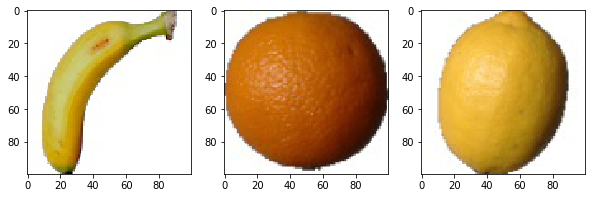
\includegraphics[width=\textwidth]{imgs/dataset_sample.png}
    \caption{Ejemplos de cada fruta obtenidos de Fruit 360}
    \label{fig:dataset_sample}
\end{figure}

\subsubsection{Dataset propio}

Posteriormente y luego de haber elegido las características a elegir se probaron los algoritmos desarrollados con fotografías propias, totalmente distintas a las de Fruits 360. 

Se tomaron imágenes de bananas, naranjas y limones de forma casera con la ayuda de un celular Huawei P9. El setup consistió de un reflector LED de 10W de luz blanca fría que iluminaba a la fruta en cuestión sobre un fondo blanco. Se utilizó esta fuente de luz porque las luces comunmente encontradas en las casas no proveen suficiente intensidad lumínica además de que poseen demasiada dispersión y generalmente son de un color blanco cálido. El flash del celular tenía el problema de ser demasiado puntual por lo que generaba zonas mal iluminadas en las esquinas de la imagen. Además se tomaron las fotografías ajustando el ISO y aumentando el tiempo de obturación para que más luz ingrese al sensor de la cámara y de esta forma obtener un fondo con un color más cercano al blanco puro. Esto es para poder realizar un \textit{thresholding} más óptimo y de esta forma separar mejor el \textit{background} del \textit{foreground}, la fruta. La resolución de las fotos es de 3000x3000 = 9MP. Por último, es valioso aclarar que las fotos fueron tomadas con un sensor monocromático por lo que no fue necesaria la transformación de RGB a escala de grises. Sin embargo sí se tuvo que transformar la escala de valores de los pixeles de la imagen: de números enteros de 0 a 255 (8 bits) a números en punto flotante de 0 a 1. 

La cantidad de imágenes en el dataset propio es mucho menor ya que estas se usaron únicamente para testear los algoritmos. Además debido a que la resolución de las fotos es significativamente más grande que la de las frutas de Fruits 360 el tiempo de ejecución aumentó notablemente por lo que se decidió mantener un número bajo de imágenes. En un trabajo futuro se podrían explorar algoritmos para hacer \textit{downscaling} y evaluar su efecto en el rendimiento.

\subsection{Filtrado y acondicionamiento de imagen}
\label{sec:filter_thresh}

Como uno de los requerimientos es analizar las imágenes en escala de grises, se cargan todas las imágenes del dataset con la ayuda de un método de \textit{skimage} y se obtienen las imágenes como se observa en la figura \ref{fig:dataset_sample_gray}.

\begin{figure}[h]
    \centering
    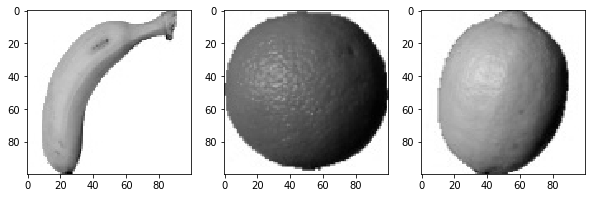
\includegraphics[width=\textwidth]{imgs/dataset_sample_gray.png}
    \caption{Ejemplos cargados en escala de grises }
    \label{fig:dataset_sample_gray}
\end{figure}{}

\subsubsection{Filtro gaussiano}

Luego se hicieron experimentaciones tratando las imágenes en \textit{raw}, es decir, sin ningún tipo de filtrado. Esto funcionó bien para el dataset \textit{Fruits 360} ya que este viene preprocesado y el \textit{background} ya está bastante bien separado del objeto. Cuando se comenzó el análisis con el dataset propio comenzaron los inconvenientes. Estas imágenes, aunque \textit{a priori} no parecían tener ningún problema, tenían cierta cantidad de ruido que afectaba la performance de los algoritmos de \textit{thresholding} que se explican luego en la sección \ref{subsec:thresholding} y consecuentemente la performance de los algoritmos \textit{k-means} y \textit{k-nn} se veía disminuida.

Es por esto que se decidió aplicar un filtro para mitigar el ruido que poseen las fotos. Se usó un filtro gaussiano con una desviación estándar igual al 0.5\% de la cantidad horizontal de pixeles de la imagen. Este valor es paramétrico ya que los distintos datasets tienen imágenes de diferentes resoluciones. Así se obtiene que para las imágenes de \textit{Fruits 360} $\sigma = 0.5$ y para el dataset propio, $\sigma = 15$. 

\subsubsection{Thresholding}
\label{subsec:thresholding}

En primera instancia se intentó hacer la clasificación teniendo realizando un análisis textural de las imágenes en escala de grises. Esto significa que cada pixel de la imagen tendrá una ponderación distinta y esta será un número de punto flotante de 0 a 1. Viéndolo desde un punto de vista mecánico, cada pixel tiene una masa distinta y hay regiones de la imagen que tienen distintas densidades. Sin embargo este enfoque no resultó en una buena clusterización de los datos, lo que implicó un muy mal desempeño de los algoritmos.

Es por esto último que se optó por dar un paso más y binarizar la imagen. De esta forma todos los pixeles que son parte del objeto a analizar tienen un valor de 1 (blanco puro) y el fondo o \textit{background} un valor de 0 (negro puro).

Para realizar este proceso existen varios algoritmos que realizan el thresholding de forma automática y adaptativa. La librería \textit{scikit-image} provee implementaciones para varios, entre ellos \textit{Isodata}, \textit{Otsu}, \textit{Mean}, \textit{Triange} y más. Además cuenta con una función en la que se pueden evaluar rápidamente los resultados para distintos algoritmos. Luego de evaluar la performance de estos se eligió como algoritmo el método \textit{Triangle}. Aunque este no presentó el mejor rendimiento en el dataset propio, sí tiene un comportamiento muy aceptable y consistente entre todas las frutas del dataset \textit{Fruit 360}. Otras opciones, como \textit{Otsu} o \textit{Minimum}, que tenían una performance excelente con bananas, fallaban en gran medida con limones. Como ya se mencionó, antes de aplicar el \textit{threshold} a la imagen se le aplicó un filtro gaussiano. En la figura \ref{fig:orig_gauss_thresh} se puede apreciar este método.


\begin{figure}[h]
    \centering
    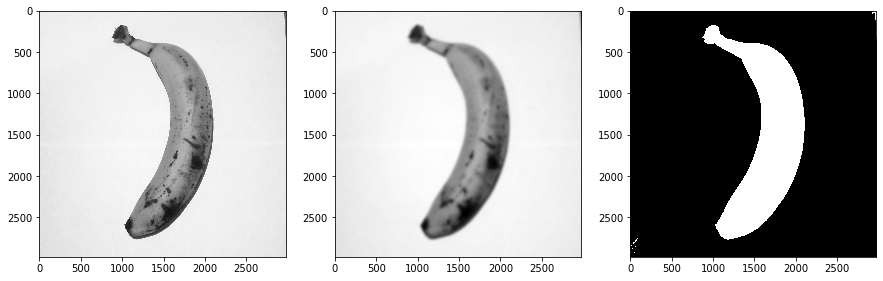
\includegraphics[width=\textwidth]{original_gauss_thresh_banana.png}
    \caption{Banana ejemplo del dataset propio. A la izquierda, la foto original. En el centro, luego de pasar por un filtro gaussiano con $\sigma = 30$. A la derecha el algoritmo \textit{Triangle threshold} aplicado a la figura del centro.}
    \label{fig:orig_gauss_thresh}
\end{figure}

\subsection{Extracción de características}

Luego del procesamiento de las imágenes detallado anteriormente, se debe realizar la extracción de características. Debemos encontrar un valor o un conjunto de valores que sean representativos de cada imagen para poder usarlos como datos de entrada a los algoritmos implementados. 

Muchas técnicas distintas existen para poder extraer características de una imagen. Ya que en la sección \ref{sec:filter_thresh} se obtuvo una imagen binaria de cada fruta, tenemos información acerca de la \textit{forma} de cada fruta. Es por esto que en este trabajo se decidió aplicar un enfoque geométrico para obtener las características.

\subsubsection{Relación de Inercia}

Dado que las tres frutas en cuestión tienen formas bastante diferentes entre sí, se supuso que sus tres momentos de área deben ser lo suficientemente distintos como para distinguirlas entre sí. Primero se pensó en los momentos de la imagen respecto a los ejes que crean la fila cero y la columna cero pero estos valores no son invariantes respecto a la translación, por lo que la ubicación de la fruta en la foto impactaría mucho. La solución es encontrar los momentos centrales o centroidales en los dos ejes, horizontal y vertical. Estos son invariantes respecto a la translación pero  no respecto a la rotación. Además estos dos parámetros son función de la cantidad de pixeles de la imagen, lo que supone un gran problema. Esto último se soluciona calculando los momentos centroidales normalizados, pero aún así no se obtiene una característica que sea invariante a la rotación, translación y la escala de la fruta. 

Finalmente se calculó el tensor de inercia de la imagen. Los autovalores de esta matriz indican las magnitudes de los momentos principales de inercia y los correspondientes autovectores indican la dirección de los ejes principales de inercia. Aunque los autovalores de la matriz son función de la escala de la imagen, no lo es el cociente entre ellos. Definimos como relación de inercia al cociente entre el mayor momento principal y el menor. De esta forma, la relación de inercia da una estimación del alargamiento de la fruta analizada. Para las naranjas, dado que su forma asemeja una esfera, se espera una relación de inercia cercana a la unidad. Para los limones, siempre que las fotografías se tomen en un plano paralelo al eje del limón, se esperan valores superiores a la unidad. Por último, para las bananas, se espera que la relación de inercia sea la máxima de las tres. 

En la figura \ref{fig:hist_inertia_ratio} se observa un histograma de las relaciones de inercia para las distintas frutas. Si bien se ve una buena diferenciación entre naranjas y limones, las bananas presentan mucha dispersión en sus valores y se observa cierta interferencia con los valores de los limones.

\begin{figure}[h]
    \centering
    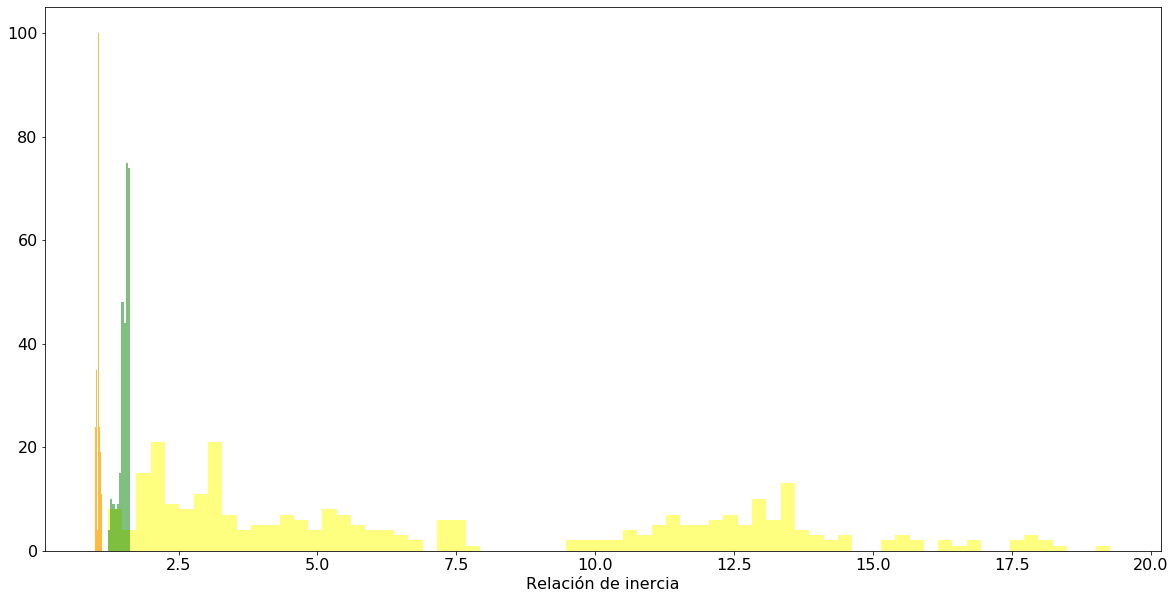
\includegraphics[width=1\textwidth]{histogram_inertia.png}
    \caption{Histograma de las relaciones de inercia para las distintas frutas. Naranjas en color naranja, limones en verde y bananas en amarillo}
    \label{fig:hist_inertia_ratio}
\end{figure}

Aunque se quiso utilizar la relación de inercia como una de las características, se observó en la implementación que su introducción empeoraba el rendimiento del agente. Es por esto que se deja la exploración de este análisis para trabajos futuros.

\subsubsection{Hu Moments}

Otra alternativa fue utilizar los \textit{Hu moments}. Estos son un grupo de 7 valores propuestos por Hu \cite{Hu1962} \cite{Huang} que son invariantes a la translación, rotación y escala de la imagen. Estos se calculan en función de los momentos centroidales del objeto. 

Los valores y las escalas de los 7 Hu moments son muy distintos entre sí, con diferencias de hasta 3 o 4 órdenes de magnitud entre ellos y escalas en el orden de $10^{-12}$ o $10^{-14}$. Es por esto que se aplica una transformación logarítmica para que los valores sean comparables entre ellos y que además las escalas de los números sean más apreciables para un humano. 

\begin{equation*}
    H_i = -sign(H_i)*log_{10}(abs(H_i))
\end{equation*}

De esta forma se obtuvieron los histogramas para las 7 componentes (de 0 a 6) de los Hu moments para el conjunto de training de \textit{Fruits 360}. Esto se observa en la figura \ref{fig:hist_hu}. Queremos elegir como características aquellas componentes que presenten la mayor separación entre las frutas, es decir, que nos permitan clusterizar de una mejor forma el dataset.

\begin{figure}[h]
    \centering
    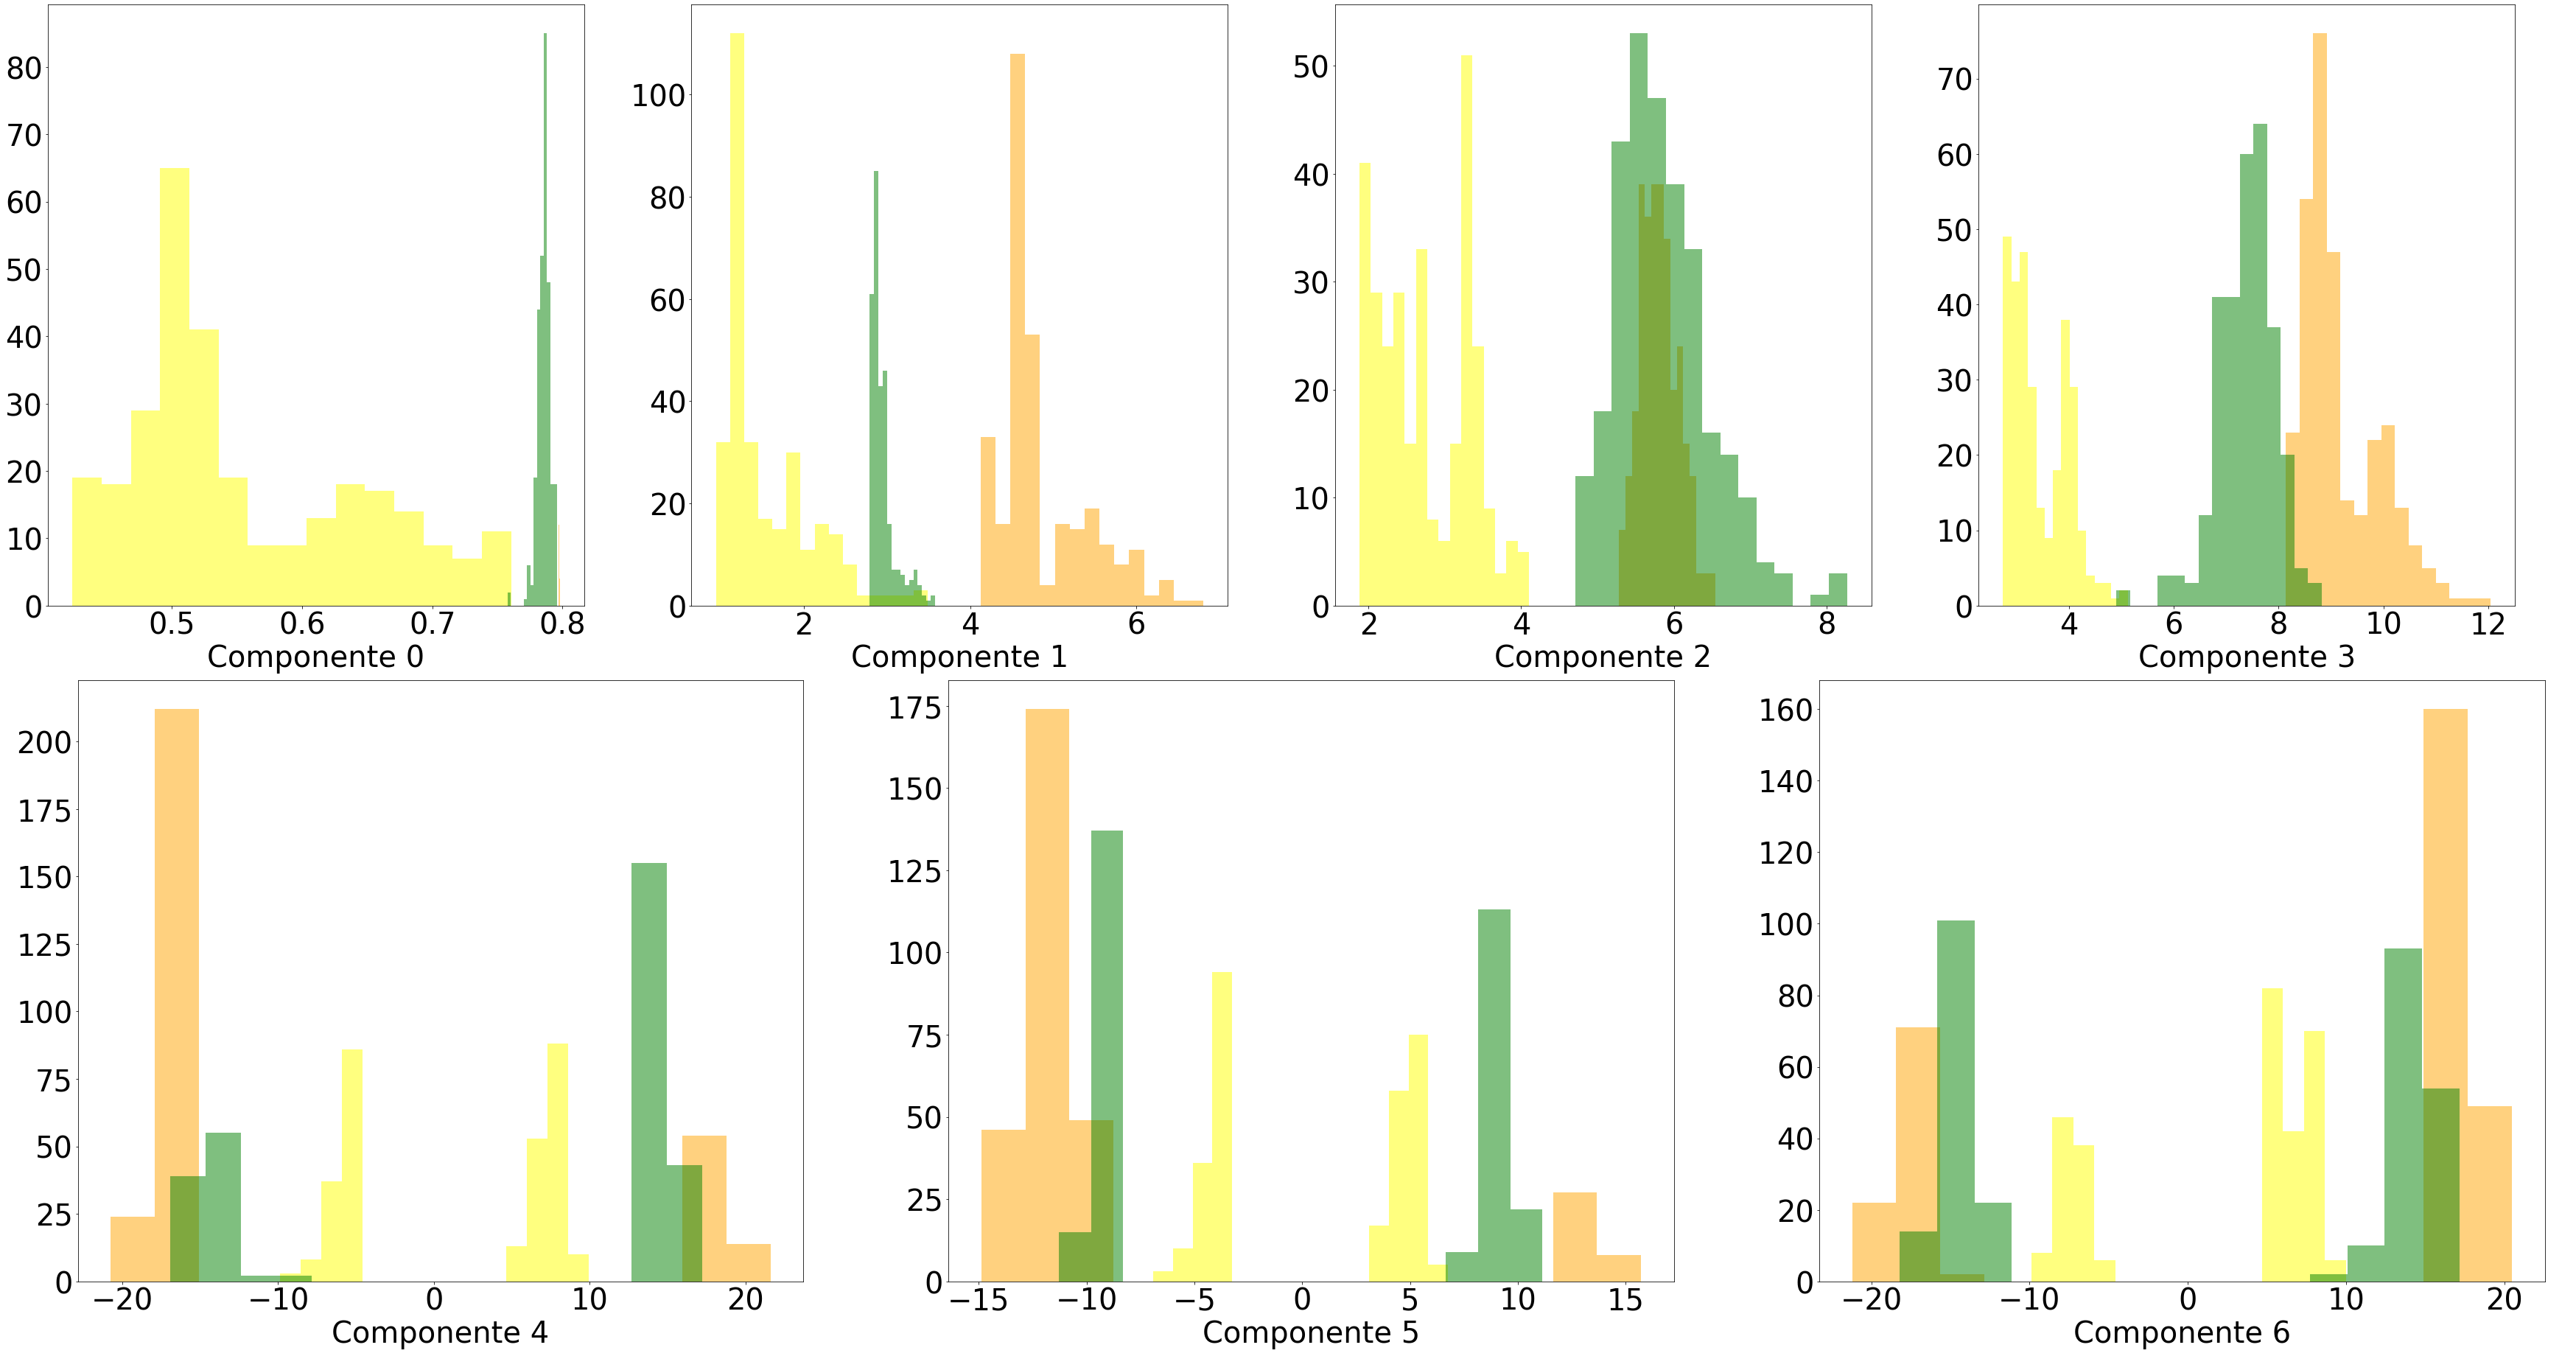
\includegraphics[width=\textwidth]{histogram_hu.png}
    \caption{Histograma de los Hu moments para las frutas de Fruits 360. Colores como en la figura \ref{fig:hist_inertia_ratio}. Componentes de 0 a 6, nótese la buena separación en las componentes 1 y 3.}
    \label{fig:hist_hu}
\end{figure}

Se observa que las componentes 1 y 3 presentan una buena separación de las frutas, por lo que se decide tomar estas dos como características para representar cada imagen. En la figura \ref{fig:means_comparison} se observa el resultado de ubicar en un plano x-y cada fruta del set de training de Fruits 360 y la clusterización con \textit{k-means}.


\subsection{Algoritmos}

\subsubsection{K-means}

\textit{K-means} es un algoritmo de clustering en el que se intenta particionar n observaciones en k clusters, en el cual cada observación pertenece al cluster con el centroide (o media) más cercano. 

El algoritmo se puede resumir en los siguientes pasos: 

\begin{enumerate}
    \item Elegir la cantidad de clusters k;
    \item Elegir aleatoriamente k puntos, que serán los centroides semilla;
    \item Asignar cada punto al centroide más cercano;
    \item Computar y ubicar el nuevo centroide de cada cluster;
    \item Reasignar cada observación al nuevo centroide más cercano. Si hubo alguna reasignación, repetir el paso anterior. Si no, el modelo está listo y se encuentra en un mínimo. 
\end{enumerate}

El modelo está plenamente definido con la ubicación de los k centroides por lo que una vez calculados, las nuevas asignaciones son muy rápidas. Si se quiere asignar un nuevo punto hay que calcular las distancias en espacio de características a los centroides y el nuevo punto pertenecerá al cluster más cercano. Podemos decir que una vez finalizado el cálculo del modelo, \textit{k-means} es muy eficiente en cuanto a tiempo de ejecución y memoria. Este algoritmo no asegura la optimalidad de la solución; dependiendo de los centroides semilla la solución puede terminar en un mínimo local que no caracterice fielmente el dataset. Esto se puede observar en la figura \ref{fig:means_comparison}.

Para evitar este problema se decidió que cada uno de los tres centroides semilla pertenezcan a cada uno de los tres tipos de fruta. Aunque esta no es una implementación \textit{vanilla} del algoritmo, evita de gran manera caer en situaciones como la que se observa en la figura \ref{fig:means_comparison} der. Como la clase de cada fruta del set de training es conocida, no tiene sentido elegir tres al azar y esperar que el algoritmo converja a un resultado favorable cuando se puede ``ayudar'' al algoritmo y mejorar la performance. Naturalmente, en datasets sin etiqueta esto no se puede realizar. 

Otro dato a destacar es que este algoritmo no hace uso de las \textit{labels} de los datos (salvo en lo detallado en el párrafo anterior), sino que únicamente los agrupa por cercanía en espacio de características. Para poder realizar una clasificación, lo que se hizo en este trabajo es tomar los clusters generados y, por voto de la mayoría, elegir la \textit{label} del cluster como se detalla en el cuadro \ref{tab:k_means_clusters}. De esta forma, en la figura \ref{fig:means_comparison} izq. se puede ver el cluster rojo que está compuesto mayoritariamente por bananas, el azul por limones y el verde por naranjas.  

\begin{figure}[h]
    \centering
    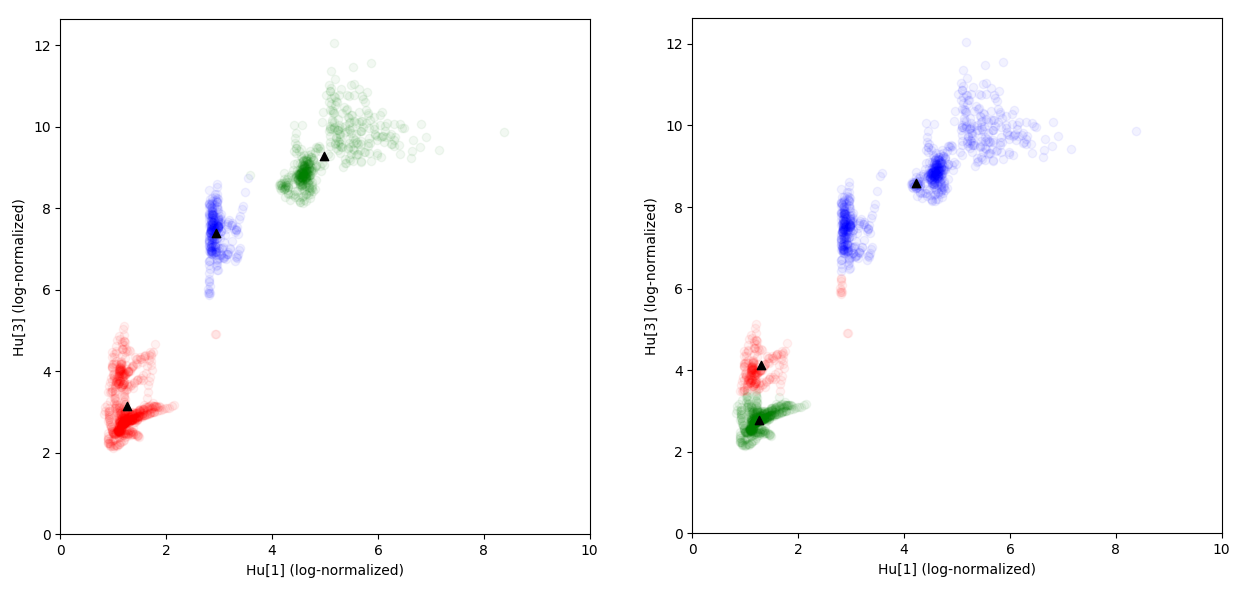
\includegraphics[width=\textwidth]{means_cluster_comparison.png}
    \caption{Efecto de la aleatoriedad de los centroides semilla para Fruits 360. A la izquierda se ve una clusterización fiel a los datos de entrada. A la derecha se observa una configuración en un mínimo local no representativa de los datos. En la figura de la izquierda, en rojo el cluster asignado a bananas, en azul el de limones y en verde el de naranjas. Además se observan los centroides de cada cluster.}
    \label{fig:means_comparison}
\end{figure}


\subsubsection{K-nn}

El algoritmo \textit{k-nearest neighbours} o \textit{k-nn} es un algoritmo de inteligencia artificial utilizado para clasificación y regresión. Usado para clasificar, consiste en ubicar cierta cantidad de observaciones en espacio de características (o \textit{feature space}) junto con su respectiva etiqueta. Luego, a cada una de las nuevas observaciones sin etiqueta le será asignada una clase en base a los k vecinos más cercanos. Existen distintas formas de ponderar las contribuciones de los k vecinos; una de ellas es tomar $1/d$ como coeficiente u otra más sencilla, es tomar a cada vecino con una contribución de 1. De esta forma, la clase es asignada por voto de la mayoría. Este enfoque es el utilizado en este trabajo.

Dado que para cada fruta a la cual se le requiere asignar su clase hay que calcular la distancia en espacio de características con todos las frutas del set de training, este algoritmo resulta más ineficiente en términos de tiempo de ejecución que \textit{k-means} si el set de training es muy grande. El tiempo crece linealmente con la cantidad de ejemplos en el set de training y además hay que realizar un ordenamiento para elegir los k vecinos más cercanos. De acuerdo al algoritmo utilizado para el \textit{sorting} puede variar la complejidad de \textit{k-nn}. Para datasets muy grandes el tiempo de cálculo de distancias puede tornarse excesivamente largo.

Se evaluaron distintas cantidades de vecinos pero no se encontraron grandes diferencias en la performance. Se decidió tomar 20 vecinos ya que esta cantidad generaba resultados aceptables. Una exploración más exhaustiva de este hiperparámetro se deja como trabajo a futuro.

\section{Resultados}

\subsection{K-means}

En la primera parte del algoritmo \textit{k-means} se generan los clusters a partir del conjunto de training de \textit{Fruits 360}. Se ubican todas las frutas en espacio de características como se observa en la figura \ref{fig:means_comparison}. A cada cluster se le asigna la clase de acuerdo al voto de la mayoría, es decir, si en cierto cluster hay mayoría de bananas entonces se lo etiqueta como un cluster de bananas. De esta forma quedan conformados los clusters A, B y C como se ve en el cuadro \ref{tab:k_means_clusters}. Esta es la etapa de entrenamiento o \textit{training} y los datos aquí obtenidos se consideran \textit{ground truth}.

\begin{table}[h]
\caption{Etapa de training de \textit{k-means}. Cantidad de frutas en cada cluster y los respectivos centroides. Por voto de la mayoría, se asigna una clase a cada cluster.}
\begin{center}
\begin{tabular}{|l|c|c|c|}
\hline
\multirow{2}{*}{}  & \multicolumn{3}{c|}{Clusters}                          \\ \cline{2-4} 
                   & A                & B                & C                \\ \hline
Bananas            & 298              & 0                & 0                \\ \hline
Naranjas           & 0                & 304              & 0                \\ \hline
Limones            & 0                & 3                & 293              \\ \hline
Centroide          & {[}1.60; 3.54{]} & {[}5.07; 9.03{]} & {[}2.99; 7.64{]} \\ \hline
Identificado como: & `banana'         & `orange'         & `lemon'          \\ \hline
\end{tabular}
\label{tab:k_means_clusters}
\end{center}
\end{table}

Las asignaciones de las frutas de los conjuntos de test se hacen en base a las medias obtenidas a partir del conjunto de training. De esta forma, se observa en el cuadro \ref{tab:k_means_test_results} el desempeño del algoritmo evaluándolo con los sets de test de \textit{Fruits-360} y con el dataset propio. Este último nunca fue utilizado para entrenar y es por lo tanto información totalmente nueva para el algoritmo. Es decir, se evalúa el desempeño con imágenes muy distintas a las utilizadas para entrenar. Aún así se obtienen buenos resultados aunque se debería aumentar la cantidad de imágenes del dataset propio para tener más fuerza estadística. La efectividad se calcula como la cantidad de aciertos (asignaciones correctas) sobre el total de imágenes.

Como se explicó, el cuadro \ref{tab:k_means_test_results} muestra cuántas frutas de cada clase se han asignado a cada cluster. El set de test de \textit{Fruits-360} muestra una altísima efectividad por la gran similitud que hay entre entre las imágenes de training y las de test. El dataset propio contiene imágenes ``desconocidas"" y con el adicional de haber sido tomadas de forma casera por lo que nunca se esperaría un rendimiento del 100\%, sino siempre menor.

\begin{table}[h]
\begin{center}
\caption{Etapa de test de \textit{k-means}. Se observa la cantidad de frutas de cada clase asignado a cada cluster. Por ejemplo, se observa que para el dataset propio, en el cluster \textit{C: lemon} se han asignado hay 2 naranjas y 14 limones. La designación \textit{A}, \textit{B}, \textit{C} es consistente con el cuadro \ref{tab:k_means_clusters}.}

\begin{tabular}{|c|c|c|c|c|c|}
\hline
                                   &          & A: `banana' & B: `orange' & C: `lemon' & Efectividad             \\ \hline
\multirow{3}{*}{Fruits-360 (test)} & Bananas  & 166         & 0           & 0          & \multirow{3}{*}{100\%}  \\ \cline{2-5}
                                   & Naranjas & 0           & 160         & 0          &                         \\ \cline{2-5}
                                   & Limones  & 0           & 0           & 164        &                         \\ \hline
\multirow{3}{*}{Dataset propio}    & Bananas  & 16          & 0           & 0          & \multirow{3}{*}{91.7\%} \\ \cline{2-5}
                                   & Naranjas & 0           & 14          & 2          &                         \\ \cline{2-5}
                                   & Limones  & 2           & 0           & 14         &                         \\ \hline
\end{tabular}
\label{tab:k_means_test_results}
\end{center}
\end{table}

\subsection{K-nn}

En este algoritmo también existe una etapa de training. En ella se tiene que generar, igual a como se explicó anteriormente, un mapa de características en el cual se ubican todas las frutas del set de training de \textit{Fruits-360}. Nuevamente esta clasificación es considerada como \textit{ground truth} y a partir de ella se clasificarán las frutas del conjunto de test de \textit{Fruits-360} y del dataset propio. La asignación se realiza en base a los 20 vecinos más cercanos. Este número fue encontrado empíricamente pero no se realizó un estudio extensivo del mismo. Esto se deja como trabajo a futuro.

Los resultados se observan en el cuadro \ref{tab:k_nn_results}.

\begin{table}[h]
\begin{center}
\caption{Etapa de test de \textit{k-nn}. Se observa a qué clase se asignaron las frutas de cada dataset. Por ejemplo, de las 16 naranjas del dataset propio, 15 fueron categorizadas correctamente y una fue identificada como limón.}
    
\begin{tabular}{|c|c|c|c|c|c|}
\hline
\multirow{2}{*}{}                  & \multirow{2}{*}{} & \multicolumn{3}{c|}{Identificado como} & \multirow{2}{*}{Efectividad} \\ \cline{3-5}
                                   &                   & Banana      & Naranja      & Limón     &                              \\ \hline
\multirow{3}{*}{Fruits-360 (test)} & Bananas           & 166         & 0            & 0         & \multirow{3}{*}{100\%}       \\ \cline{2-5}
                                   & Naranjas          & 0           & 160          & 0         &                              \\ \cline{2-5}
                                   & Limones           & 0           & 0            & 164       &                              \\ \hline
\multirow{3}{*}{Dataset propio}    & Bananas           & 16          & 0            & 0         & \multirow{3}{*}{89.6\%}      \\ \cline{2-5}
                                   & Naranjas          & 0           & 15           & 1         &                              \\ \cline{2-5}
                                   & Limones           & 4           & 0            & 12        &                              \\ \hline
\end{tabular}
\label{tab:k_nn_results}
\end{center}
\end{table}

Sorpresivamente los resultados son muy similares a aquellos del algoritmo \textit{k-means}, con un solo acierto menos de diferencia. Esto indicaría que la naturaleza de los datos aquí analizados son favorables para cualquiera de los dos algoritmos analizados. Es por eso que se deben tener en cuenta otros factores a la hora de elegir uno de los algoritmos. 

Como se explicó anteriormente, una vez realizado el training, \textit{k-means} presenta una gran performance en tiempo de ejecución y en memoria. Esto es porque todo el modelo queda representado en los k centroides de los k clusters. Así es que para cada nueva asignación, solo hay que calcular k distancias y la menor de ellas definirá la clase. Por otro lado, \textit{k-nn} tiene el mismo \textit{overhead} a la hora del training pero además, a la hora de las asignaciones, debe realizar n cálculos. Siendo n la cantidad de ejemplos del dataset de training, si no hay una suficiente capacidad de cómputo a disposición, este algoritmo tendrá una performance muy inferior en tiempo de ejecución siempre que la cantidad de ejemplos sea mayor a la cantidad de clusters, lo cual es algo común. Además hay que tener en cuenta que el modelo queda caracterizado con todos los ejemplos del dataset de training y no solo con unos pocos centroides. Esto genera un uso de memoria mayor. Sin embargo \textit{k-nn} tiene un desempeño superior cuando las frutas no están claramente dentro de un cluster sino en los exteriores. En este caso \textit{k-means} tiende a generar clusters del mismo tamaño por lo que el rendimiento cae cuando hay ejemplos que caen en la periferia de un cluster. 

Por estas razones es que se recomienda utilizar \textit{k-means} para aplicaciones en las que no se tenga una gran capacidad de cálculo o que se deban hacer en un tiempo muy pequeño. Cuando los recursos no son problema se aconseja el uso de \textit{k-nn} ya que presenta mejores resultados en ejemplos ubicados en zonas de interfaz de clusters.

De esta forma se conluye que para una caja de supermercado el uso del algoritmo \textit{k-means} es el óptimo ya que posee buena efectividad, no se necesita hardware muy potente y, sobre todo, puede dar un resultado en un tiempo muy bajo. Esta característica es crucial en este entorno. \textit{K-nn} también podría implementarse pero requiere una mayor inversión en equipamiento. 

\section{Conclusión}

En este trabajo se diseñó un agente inteligente capaz de identificar y clasificar frutas entre bananas, naranjas y limones. En la primera sección se da una clasificación formal del agente especificando la tabla REAS y las propiedades del entorno de la tarea. El agente actúa sobre dos datasets, uno es \textit{Fruits 360} y el otro es un dataset propio. Luego se explican los métodos utilizados para filtrar las imágenes y realzar características de las mismas. Se utilizó un filtro gaussiano y posteriormente un \textit{thresholding} con el algoritmo \textit{Triangle}.

A la hora de elegir las características a extraer se avanzó primero en un método geométrico en el cual se utilizaba la relación de los momentos principales de inercia para evaluar el ``alargamiento" de las frutas. Este enfoque se debió abandonar ya que no generó buenos resultados pero se decidió documentar igual debido a su sencillez y la posibilidad de expandirlo en trabajos futuros. El enfoque finalmente utilizado es también geométrico y usa los Hu moments. Las componentes 1 y 3 presentaron la mejor clusterización por lo que estos dos valores fueron usados para representar cada imagen. 

Luego se explicó la implementación de los algoritmos y los resultados obtenidos. La performance de ambos fue muy satisfactoria obteniendo una efectividad del 100\% para las frutas de \textit{Fruits 360} y alrededor de 90\% para las del dataset propio. Como no se encontraron diferencias significativas en los desempeños la decisión de utilizar uno u otro dependerá de las características particulares de la implementación. Para aquellas en las que no haya disponible mucha capacidad de cómputo ni memoria se recomienda utilizar \textit{k-means} por su bajo impacto en ambas variables. Si el procesamiento y la memoria no son problema se recomienda \textit{k-nn} ya que tiene un desempeño ligeramente superior en ejemplos que no encajan perfectamente en un cluster.

Dado que el agente debe implementarse en una caja de supermercado y en este entorno el tiempo de ejecución y el bajo costo son características cruciales, se recomienda el uso de \textit{k-means}.

\printbibliography

\end{document}

